\newpage
\begin{tcolorbox}

	\lettrine{T}{here} were mixed feelings at the end of \emph{Pivo Moz}: success in metres gained (2,267m in total) was somewhat marred by the logistical costs with which it had been achieved. The exciting exploration fronts, which had remained within reasonable distance from Camp were now written off or pushed to their conclusion. The other leads lay further than ever before: either near the very deep end (\emph{Watership Down}) or a great caving distance to the south (\emph{Choke-a-Bloke} and its purported connection to the surface).

	Getting novices to navigate and successfully explore the cave is a particularly good metric to assess the outcome of an expedition: it means new members have acquired a vast set of skills they can learn nowhere else: bolting, rigging, surveying. These skills put in practice during the academic year, and subsequent expeditions play a major role in the long term survival of the club: they refresh the pool of knowledge. We will not go far wrong by saying that the baggage of experience and skills one brings back from deep alpine exploration is transferrable to many other aspects of life, but also rich and unique.

	For that reason, the format of the 2016 expedition was heatedly discussed soon after we came back to the UK but we were in a tricky situation. Wondering how best to readjust our aims and targets without losing the opportunity to find new passage, we started looking beyond \emph{Vrtnarija}, to potential new areas of the mountain, and toyed with the idea of abandoning the underground camp. Luckily, a solution presented itself, but it came in the form of a celebratory message from a well known corner of the Alps...

	The long awaited connection between \emph{Monatip -Primadona} and \emph{System Migovec} was forged during the usual October Super Action run by the JSPDT. Navigating through a system of shallow, horizontal galleries filling an area of mountain hitherto unexplored, the lucky explorers unexpectedly connected with the SE end of NCB passage, thus confirming \emph{Sistem Migovec}'s status as longest cave in ex-Yugoslavia.
	\\
	\\
	\\
	
	
\end{tcolorbox}
	\backgroundsetup{	scale=1,
					color=black,
					opacity=1,
					angle=0,
					contents={%
  						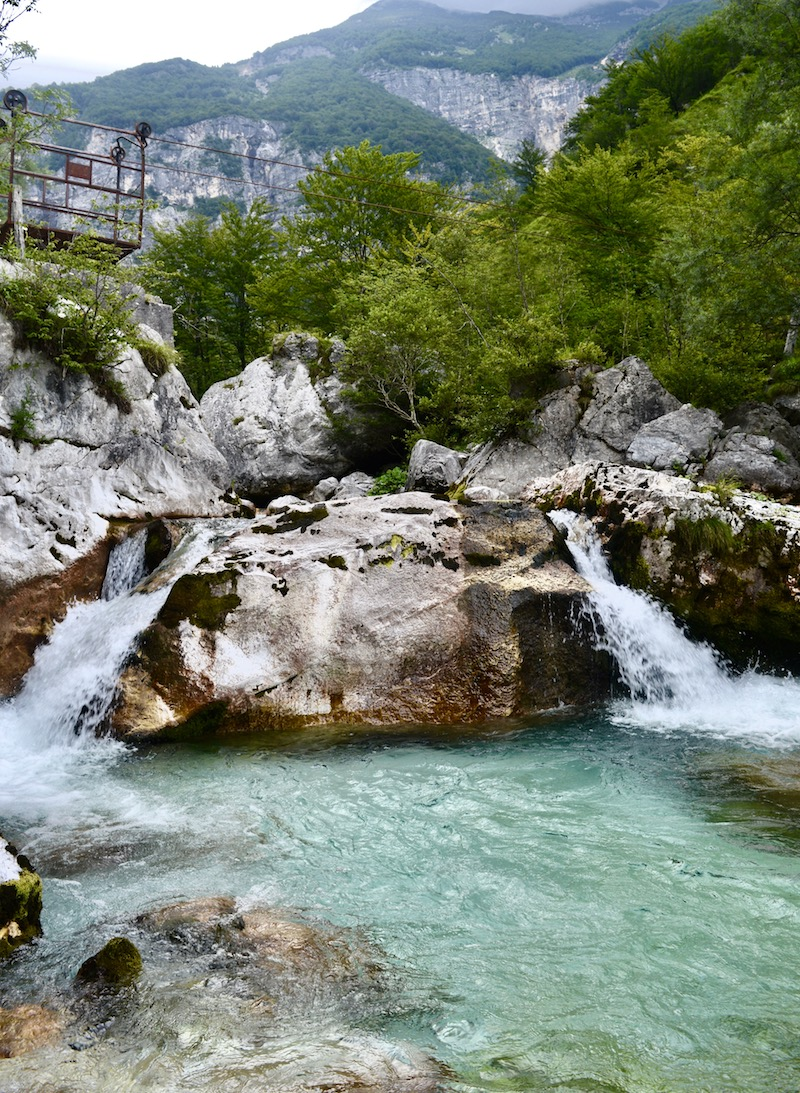
\includegraphics[height=\paperheight]{images/backgrounds/Tolminka_at_crossing__2_.jpg}
  					}
	}
\BgThispage